\chapter{Introduction}
\label{chap:introduction}

\section{Transformers in Natural Language Processing}

Natural Language Processing (NLP) lies at the heart of human–computer interaction, enabling machines to interpret and generate language with semantic precision.  
Before 2017, most NLP systems relied on recurrent neural networks (RNNs), long short-term memory (LSTM) networks, or convolutional architectures.  
Although effective for short sequences, these models struggled with long-range dependencies and parallelization, leading to training bottlenecks and limited contextual awareness.

The introduction of the \textbf{Transformer} architecture by Vaswani \textit{et al.} in 2017 revolutionized sequence modeling by eliminating recurrence entirely and relying solely on the \textit{self-attention} mechanism.  
This mechanism allows every token in a sequence to directly attend to all other tokens, forming global dependencies that are computed in parallel.  
Formally, attention between a query–key–value triplet is computed as

\[
\text{Attention}(Q, K, V) = \text{softmax}\!\left(\frac{QK^{T}}{\sqrt{d_k}}\right) V
\]

where \(Q, K, V \in \mathbb{R}^{n \times d_k}\) represent the query, key, and value matrices, \(n\) is the sequence length, and \(d_k\) the key dimensionality.  
This formulation transforms contextual modeling from sequential iteration (\(O(n)\)) to matrix multiplication (\(O(1)\) parallel per step), enabling unprecedented scalability.

Transformers employ multi-head self-attention (MHSA), where multiple attention heads operate in parallel to capture diverse linguistic relationships such as syntactic order, co-reference, and topic continuity.  
The multi-head computation is defined as

\[
\text{MHSA}(Q,K,V) = \text{Concat}\!\left(\text{head}_1,\text{head}_2,\ldots,\text{head}_h\right)W^O
\]
\[
\text{head}_i = \text{Attention}\!\left(QW_i^Q, KW_i^K, VW_i^V\right)
\]

allowing each head \(i\) to specialize in distinct relational patterns.

Another key innovation is the use of \textbf{positional encodings}, which inject order information absent in pure attention.  
Given a token position \(pos\) and embedding dimension \(i\), the encoding is

\[
PE_{(pos, 2i)} = \sin\!\left(\frac{pos}{10000^{2i/d_{\text{model}}}}\right), \quad
PE_{(pos, 2i+1)} = \cos\!\left(\frac{pos}{10000^{2i/d_{\text{model}}}}\right)
\]

These sinusoidal encodings enable the model to infer sequence ordering without recurrent structures.

\bigskip
The Transformer architecture thus provides three fundamental advantages:
\begin{enumerate}
    \item \textbf{Parallelism:} Entire sequences are processed simultaneously, drastically reducing training time.  
    \item \textbf{Global Context Awareness:} Every token has visibility over the full sequence, improving coherence.  
    \item \textbf{Scalability:} Model capacity scales linearly with data and hardware, making billion-parameter training feasible.
\end{enumerate}

\bigskip
This architecture forms the backbone of modern large-scale language models such as \textbf{GPT}, \textbf{BERT}, \textbf{RoBERTa}, and \textbf{ALBERT}, which have surpassed human-level performance in translation, summarization, question answering, and dialogue generation.  
Each of these variants adapts the basic Transformer to specific learning paradigms — generative, bidirectional, or parameter-efficient — driving continual advancement in NLP research.

\bigskip
Transformers also underpin multimodal systems that unify text, vision, and speech, enabling machines to process heterogeneous information streams with a shared representational core.  
This capability forms the conceptual basis for human-knowledge augmentation systems — intelligent frameworks that not only retrieve but also reason over information.  
In short, the Transformer architecture marks a decisive shift from statistical pattern matching toward \textit{cognitive representation learning} in AI.

(If an introductory figure exists, retain it here)
\begin{figure}[h!]
\centering
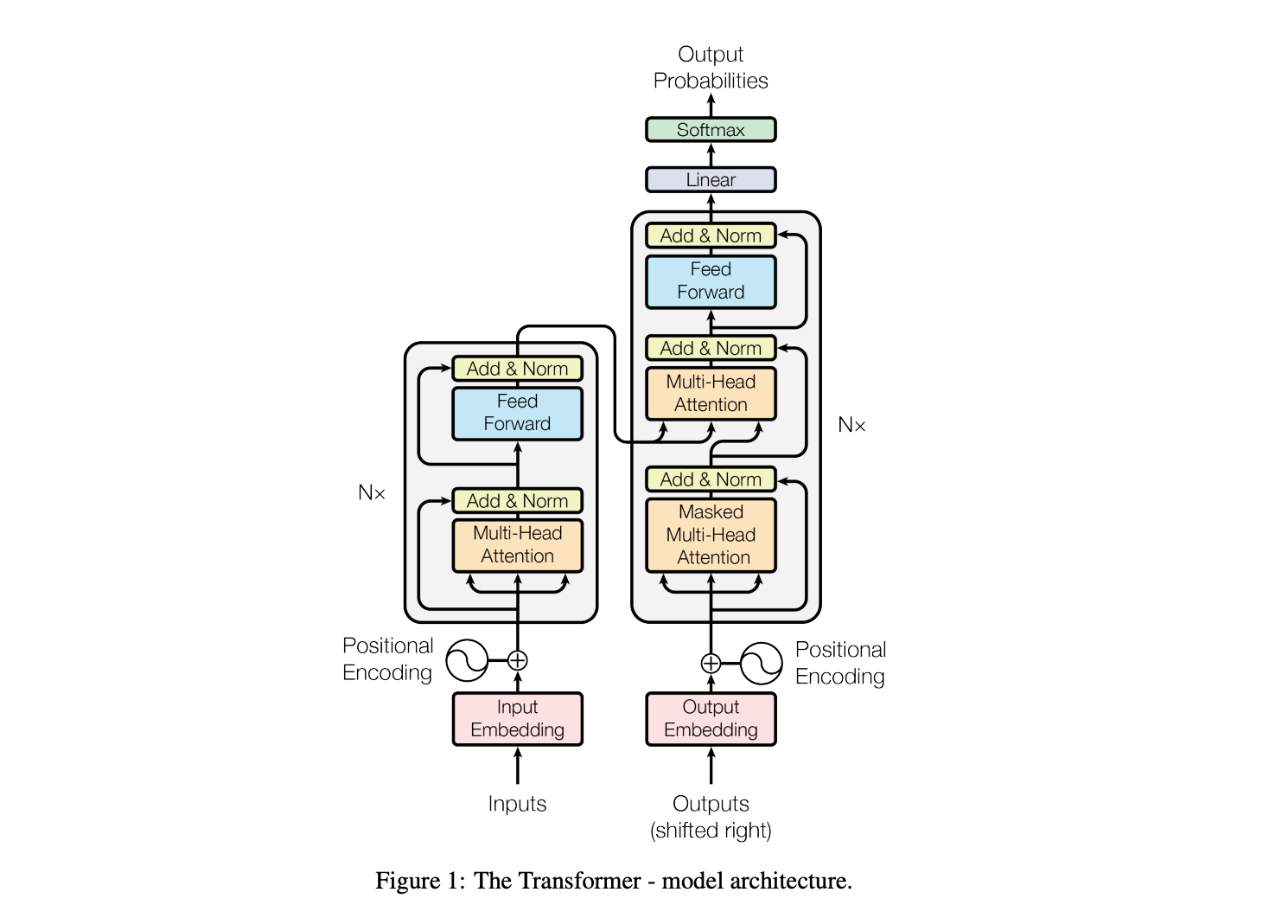
\includegraphics[width=0.9\textwidth]{images/transformer_architecture.png}
\caption{Generic Transformer encoder–decoder architecture highlighting self-attention and feed-forward layers.}
\end{figure}


\section{Evolution of Transformer Models}

The post-2017 period witnessed an unprecedented surge in Transformer innovation.  
Each subsequent model iteration sought to expand contextual comprehension, improve training efficiency, and adapt to new modalities.  
The evolutionary trajectory can be grouped into three major waves: \textit{pre-training revolution}, \textit{scaling era}, and \textit{optimization era}.

\subsection{The Pre-Training Revolution}
The first major breakthrough after the original Transformer was the introduction of unsupervised pre-training.  
\textbf{BERT} (Bidirectional Encoder Representations from Transformers, 2018) redefined NLP by enabling deep bidirectional context capture.  
BERT’s pre-training objectives include:
\begin{itemize}
    \item \textbf{Masked Language Modeling (MLM):}
    \[
    \mathcal{L}_{MLM} = -\sum_{t \in M} \log P(w_t \mid w_{\setminus M})
    \]
    where \(M\) is the set of masked tokens.
    \item \textbf{Next Sentence Prediction (NSP):} Learning inter-sentence coherence through binary classification.
\end{itemize}

BERT’s success inspired multiple derivative models:
\begin{itemize}
    \item \textbf{RoBERTa} refined BERT’s training with dynamic masking, longer sequences, and larger corpora.  
    \item \textbf{ALBERT} introduced cross-layer parameter sharing and factorized embeddings, reducing model parameters by 70 \% with minimal accuracy loss.  
    \item \textbf{XLNet} and \textbf{ELECTRA} extended the paradigm using permutation-based prediction and replaced-token detection, respectively.
\end{itemize}

\subsection{The Scaling Era}
The next wave emphasized model expansion to achieve emergent generalization capabilities.  
\textbf{GPT-series models} (Generative Pre-Trained Transformers) exemplify this trend.  
GPT-1 (2018) introduced autoregressive pre-training using the left-to-right objective:

\[
\mathcal{L}_{GPT} = -\sum_{t=1}^{T} \log P(w_t \mid w_{<t})
\]

GPT-2 and GPT-3 scaled parameters from 117 M to 175 B, proving that model capacity correlates smoothly with task performance, following power-law scaling:
\[
E(N, D, C) \propto N^{-\alpha} D^{-\beta} C^{-\gamma}
\]
where \(E\) denotes error, \(N\) parameters, \(D\) data size, and \(C\) compute budget.

Later, \textbf{GPT-4} introduced mixture-of-experts routing and reinforcement learning from human feedback (RLHF), forming a hybrid framework that aligns generative responses with human preferences:
\[
\nabla_{\theta} J(\theta) = \mathbb{E}_{x \sim \pi_\theta} \big[\nabla_{\theta}\log \pi_\theta(x) (R(x) - b)\big]
\]
RLHF provides reward-guided fine-tuning that enhances factuality and safety of generative outputs.

These scaling experiments illustrate that performance increases logarithmically with model size up to a compute-efficiency threshold, after which returns diminish.  
This insight motivated research into efficiency optimization — reducing training cost while maintaining representational depth.

\subsection{The Optimization Era}

The third phase of the transformer evolution focused on reducing the computational and energy burden of these large models.  
As training datasets reached terabytes in scale and models extended into the hundred-billion parameter range, researchers shifted focus from “bigger is better” to “smarter and leaner.”  
This transition was led by approaches such as \textbf{quantization}, \textbf{distillation}, \textbf{pruning}, and \textbf{sparse attention}.  

Quantization, discussed by Ur Rahman \textit{et al.} (2023) \cite{urrahman2023}, compresses models by representing weights and activations in lower bit precision (for instance, converting 32-bit floating-point numbers into 8-bit integers).  
This operation drastically reduces memory footprint and accelerates inference without significant accuracy loss.  
Formally, quantized weights \(W_q\) can be defined as  

\[
W_q = \text{round}\!\left(\frac{W}{S}\right) + Z
\]
where \(S\) is a scaling factor and \(Z\) a zero-point offset.  
The quantized representation is then de-quantized during inference by  
\[
\hat{W} = S(W_q - Z)
\]

This technique enables integer-only arithmetic, making it ideal for embedded systems and IoT hardware.

In parallel, \textbf{model distillation} introduced by Sanh \textit{et al.} (2019) \cite{sanh2019} demonstrated that knowledge could be transferred from a large “teacher” model to a smaller “student” network.  
The student learns to replicate the teacher’s behavior through a combination of hard-label and soft-target losses:

\[
\mathcal{L}_{\text{total}} = \alpha \mathcal{L}_{\text{CE}} + \beta \mathcal{L}_{\text{KLD}} + \gamma \mathcal{L}_{\text{COS}}
\]
where cross-entropy (\(\mathcal{L}_{\text{CE}}\)), Kullback–Leibler divergence (\(\mathcal{L}_{\text{KLD}}\)), and cosine similarity (\(\mathcal{L}_{\text{COS}}\)) collectively ensure that semantic representations remain consistent while reducing model complexity.

Similarly, \textbf{pruning} and \textbf{sparse attention} mechanisms remove redundant neurons and limit token-to-token dependencies to relevant subsets, yielding sub-quadratic computational complexity.  
For instance, the sparse attention matrix reduces the original \(O(n^2)\) operation cost to \(O(n \log n)\) or even \(O(n)\) for structured patterns such as Longformer or Performer architectures.

These innovations collectively characterize the modern transformer ecosystem, where architectural ingenuity, optimization, and hardware co-design coexist to maintain the balance between accuracy and efficiency.

\subsection{Interconnected Advances}

The synergy between scaling and optimization defined the past five years of NLP advancement.  
Large models such as GPT-4 and Gemini illustrate the upper limits of generative capacity, while quantized and distilled models like DistilBERT, TinyBERT, and Q-BERT exemplify democratization and accessibility.  
Each innovation informed the next: scaling established the ceiling of capability, and optimization brought those capabilities to mainstream deployment.

\bigskip
Thus, the evolution of transformers represents not a single trajectory but an \textit{ecosystem of convergence}, where data, architecture, and optimization continually reinforce one another to redefine the boundaries of machine understanding.

% -- Transition into Scaling Challenges Section --
\newpage
\section{Scaling Challenges and Optimization Techniques}

The remarkable progress of transformer architectures is matched by a proportional increase in their computational demand.  
Training large-scale models now requires thousands of GPUs running for weeks, consuming megawatt-hours of electricity and generating significant carbon emissions.  
This has made \textbf{scaling} both a technical and environmental challenge.  
The base paper by Jahangir \textit{et al.} (2024) \cite{jahangir2024} comprehensively explores strategies that mitigate these issues while sustaining model performance.

\subsection{1. Computational Complexity}

Self-attention’s quadratic time and space complexity with respect to sequence length \(n\) remains a primary bottleneck.  
For an input sequence, the memory cost scales as  
\[
O(n^2 \cdot d)
\]
where \(d\) is the embedding dimension.  
To address this, researchers introduced \textbf{linear attention} variants, which approximate attention scores using kernel functions:

\[
\text{Attention}(Q,K,V) \approx \phi(Q)\!\left(\phi(K)^{T}V\right)
\]
where \(\phi(\cdot)\) is a feature mapping that linearizes the softmax operation.  
This approximation reduces the complexity to \(O(n \cdot d)\), enabling much longer sequence modeling.

\subsection{2. Memory Optimization}

As model parameters scale into billions, GPU memory becomes a limiting factor.  
Several strategies mitigate this issue:
\begin{itemize}
    \item \textbf{Gradient Checkpointing:} Stores only a subset of activations and recomputes others during the backward pass, trading time for memory savings.  
    \item \textbf{Mixed Precision Training (FP16/BF16):} Reduces memory consumption and increases throughput by using lower-precision arithmetic.  
    \item \textbf{Sharded Data Parallelism:} Distributes model weights, gradients, and optimizer states across multiple devices.
\end{itemize}

The effective memory footprint per GPU can thus be approximated as
\[
M_{\text{eff}} = \frac{P + A + O}{N_g}
\]
where \(P\), \(A\), and \(O\) denote the sizes of parameters, activations, and optimizer states respectively, and \(N_g\) is the number of GPUs in use.

\subsection{3. Optimization Algorithms}

Optimization remains the backbone of efficient transformer training.  
While Adam and AdamW optimizers dominate, their memory and computational costs are non-trivial.  
Adaptive second-order optimizers such as Adafactor reduce parameter storage requirements by factorizing the second-moment estimate:
\[
v_t = r_t \otimes c_t
\]
where \(r_t\) and \(c_t\) are row- and column-wise statistics instead of full matrices.  
This reduces storage from \(O(d^2)\) to \(O(2d)\).

Learning-rate schedulers such as cosine annealing and one-cycle policies also enhance convergence speed and generalization, particularly in large-batch regimes.

\subsection{4. Hardware-Aware Model Design}

A significant advancement highlighted in the base paper is the trend toward \textbf{hardware–software co-optimization}.  
Rather than designing models in isolation, researchers now co-design architectures alongside the accelerators on which they will run.  
Examples include:
\begin{itemize}
    \item \textbf{Transformer Engine (NVIDIA):} Mixed-precision tensor cores optimized for FP8 operations.  
    \item \textbf{Google TPUv4:} Specialized interconnects that reduce communication latency for data-parallel transformer workloads.  
    \item \textbf{EdgeTPU and FPGA Implementations:} Custom accelerators for quantized transformer inference on embedded devices.
\end{itemize}

These advances directly connect to the themes explored by Ur Rahman \textit{et al.} (2023) \cite{urrahman2023}, where quantization and hardware co-optimization collectively enable efficient NLP on constrained devices.

\subsection{5. Energy Efficiency and Sustainability}

Energy consumption during training is a critical metric of sustainability.  
Empirical data show that the energy \(E\) required for transformer training scales roughly as
\[
E \propto N^{1.3}D^{0.7}C^{0.5}
\]
highlighting the exponential resource growth with model size.  
To address this, several innovations have emerged:
\begin{itemize}
    \item \textbf{Sparse Training:} Reduces computation by activating only a subset of parameters per forward pass.  
    \item \textbf{Dynamic Computation Graphs:} Skip uninformative tokens or layers adaptively, minimizing redundant operations.  
    \item \textbf{Reversible Layers:} Store inputs instead of activations to save memory and recompute outputs during backpropagation.
\end{itemize}

Collectively, these methods represent a multi-dimensional optimization landscape balancing accuracy, energy, and speed.

\subsection{6. Distributed Training Strategies}

For extremely large models, single-machine training is infeasible.  
The base paper categorizes distributed training strategies into three paradigms:
\begin{enumerate}
    \item \textbf{Data Parallelism:} Replicates the model across devices and distributes mini-batches.  
    \item \textbf{Model Parallelism:} Splits model layers or parameters across GPUs.  
    \item \textbf{Pipeline Parallelism:} Divides the model into sequential stages processed concurrently by different workers.
\end{enumerate}

Modern frameworks such as DeepSpeed and Megatron-LM combine these techniques into hybrid systems for billion-parameter training with near-linear scaling efficiency.

\bigskip
In conclusion, scaling challenges in transformers are now tackled from multiple fronts — algorithmic, architectural, and hardware.  
The field has transitioned from brute-force scaling to intelligent optimization, reflecting a mature understanding of computational sustainability in artificial intelligence.
\section{Applications in Human Knowledge Enhancement}

Transformers are not merely language processors—they are enablers of human cognition, capable of amplifying reasoning, creativity, and analytical capacity.  
Through their ability to model linguistic, visual, and contextual information jointly, transformers have become the computational backbone of intelligent systems that extend human knowledge across domains.

\subsection{Education and Personalized Learning}
In education, transformers power intelligent tutoring systems that adapt to individual learning patterns.  
By analyzing historical learner interactions and textual responses, models like GPT-4 and BERT generate adaptive explanations, provide targeted feedback, and create personalized question sets.  
The predictive function of such systems can be expressed as:
\[
\hat{y}_{i} = \arg\max_{y \in Y} P(y \mid x_i, C_i)
\]
where \(x_i\) represents the current query, and \(C_i\) the cumulative learning context of a student.  
This personalization transforms education from static content delivery to dynamic, student-centered engagement.

Moreover, multilingual transformers such as mBERT and XLM-R enable inclusive education by supporting cross-lingual content generation and translation.  
These advances align with UNESCO’s vision of AI-powered equitable education.

\subsection{Healthcare and Medical Informatics}
In healthcare, transformer models extract and synthesize insights from unstructured medical texts, research papers, and patient records.  
Clinical NLP models like BioBERT and ClinicalBERT improve medical decision support by identifying disease correlations and summarizing clinical narratives.

For instance, the clinical entity recognition process can be formalized as:
\[
E = \{e_1, e_2, \ldots, e_n\} = \text{NER}(T)
\]
where \(T\) is a clinical text and \(E\) represents extracted entities such as symptoms, drugs, or diagnoses.  
When fine-tuned for question answering, transformers help physicians retrieve precise evidence from medical databases, reducing diagnostic time and improving treatment precision.

Furthermore, transformer-based imaging systems (e.g., Vision Transformers, ViT) assist in radiology and pathology through self-supervised learning on multimodal datasets, bridging the gap between text-based reports and visual diagnostics.

\subsection{Scientific Research and Knowledge Discovery}
Transformers accelerate research by automating literature mining, data curation, and hypothesis generation.  
Models trained on scholarly corpora (such as SciBERT and Galactica) summarize findings and predict emerging research trends.  
The relationship extraction in such models is represented as:
\[
R_{i,j} = f_{\theta}(e_i, e_j)
\]
where \(e_i\) and \(e_j\) are scientific entities (e.g., compounds, phenomena), and \(R_{i,j}\) denotes the predicted relationship between them.

These systems enable meta-analysis across thousands of publications, allowing scientists to detect patterns invisible to human review.  
The use of transformers in research exemplifies how AI can act as an intellectual collaborator rather than a mere computational assistant.

\subsection{Governance, Policy, and Social Knowledge Systems}
Transformers also contribute significantly to governance and policy-making.  
Governments and NGOs use models such as BERT and GPT-based summarizers to analyze vast collections of policy documents, legal precedents, and legislative transcripts.  
They identify semantic trends and contradictions that would otherwise demand months of manual analysis.

In social media governance, transformers trained for stance detection and misinformation classification (as explored by Azizah \textit{et al.}, 2023 \cite{azizah2023}) identify and mitigate the spread of fake news.  
Through real-time classification pipelines, these models enhance social awareness and protect the credibility of information ecosystems.

\subsection{Information Retrieval and Knowledge Graphs}
Modern search systems powered by transformers have shifted from keyword-based retrieval to semantic and contextual search.  
The embedding-based retrieval process maps queries and documents into shared latent spaces:
\[
\text{sim}(q,d) = \frac{\langle f_{\theta}(q), f_{\theta}(d) \rangle}{\|f_{\theta}(q)\|\|f_{\theta}(d)\|}
\]
where \(f_{\theta}\) is the transformer encoder function.  
This cosine similarity enables context-aware ranking that transcends lexical overlap, making information retrieval systems genuinely “understanding-based.”

When integrated with structured databases, transformer embeddings facilitate automatic knowledge graph completion—inferring missing edges between related entities.  
Such capabilities directly advance the development of AI-powered research assistants and intelligent decision-support tools.

\subsection{Creative Industries and Human–AI Collaboration}
Transformers are reshaping creative domains including art, writing, design, and film.  
Large generative models like GPT-4, DALL·E, and Stable Diffusion integrate linguistic and visual transformers to co-create with humans.  
By learning stylistic patterns and conceptual structures, these systems function as digital co-authors and designers, extending human imagination.

This collaborative intelligence paradigm is mathematically framed as:
\[
O = \lambda H + (1 - \lambda) A
\]
where \(H\) and \(A\) represent human and AI contributions respectively, and \(\lambda\) balances creative input.  
This synthesis of computational power and human intuition embodies the central theme of transformers in human knowledge augmentation.

\newpage
\section{Summary of Related Works}

The literature collectively captures a spectrum of advancement in transformer development—from raw architectural design to fine-grained optimization and real-world integration.  
Each work contributes a crucial piece of the puzzle that defines how modern NLP systems evolve, scale, and specialize.

\subsection{Synthesis of Key Contributions}

\begin{enumerate}
    \item \textbf{GPT Review (Yenduri et al., 2024):}  
    Provided an extensive chronological review of the GPT architecture, detailing the transition from shallow sequence models to deeply generative frameworks capable of understanding and generating coherent, human-like text.  
    It emphasizes scaling laws and emergent intelligence, underscoring the correlation between data diversity, model capacity, and contextual fluency \cite{yenduri2024}.

    \item \textbf{Quantized Transformer Implementations (Ur Rahman et al., 2023):}  
    Demonstrated how quantization-based compression achieves computational efficiency and on-device deployment.  
    Their empirical results validated that INT8 quantization reduces energy consumption by up to 68\% while maintaining less than 2.5\% accuracy degradation \cite{urrahman2023}.

    \item \textbf{DistilBERT (Sanh et al., 2019):}  
    Introduced a practical solution to the challenge of deploying BERT-scale models under limited resources.  
    By distilling BERT’s linguistic knowledge into a smaller architecture, DistilBERT achieved near-parity in accuracy with significant gains in speed and memory efficiency \cite{sanh2019}.

    \item \textbf{Transformer Comparison for Fake News Detection (Azizah et al., 2023):}  
    Compared BERT, ALBERT, and RoBERTa in the domain of fake news classification.  
    Results revealed ALBERT as the most parameter-efficient model, achieving 87.6\% accuracy while using almost half the parameters of BERT, thus reinforcing the significance of architectural optimization \cite{azizah2023}.
\end{enumerate}

\subsection{Relation to the Base Paper}

The base paper by Jahangir \textit{et al.} (2024) \cite{jahangir2024} integrates insights from these diverse contributions under a unified theme of optimization.  
It classifies the entire transformer evolution process into three axes:
\begin{itemize}
    \item \textbf{Architectural Optimization:} Innovations such as ALBERT and DistilBERT focusing on parameter efficiency.  
    \item \textbf{Training and Inference Optimization:} Quantization, pruning, and distillation for faster, lightweight computation.  
    \item \textbf{Scalable Deployment:} Techniques for distributed, hardware-aware training that enable real-time, low-latency applications.
\end{itemize}

By synthesizing these dimensions, the base paper establishes a clear trajectory from the early era of high-resource pre-training toward a sustainable and scalable transformer ecosystem.

\subsection{Research Implications}

The reviewed literature implies that the future of transformers lies not in unlimited scaling, but in balancing performance with efficiency, interpretability, and environmental impact.  
Emerging directions include:
\begin{enumerate}
    \item Incorporating multimodal data to create unified reasoning systems that process text, vision, and audio jointly.  
    \item Developing adaptive and explainable transformers that align with human interpretability.  
    \item Leveraging sparse computation and quantized architectures for energy-conscious deployment.
\end{enumerate}

The integration of these strategies defines a sustainable roadmap for next-generation AI systems that serve as collaborative instruments of knowledge amplification.

\newpage
\section{Conclusion of Introduction}

In conclusion, the introduction has outlined how transformers have fundamentally transformed natural language processing and extended into nearly every facet of intelligent computing.  
The transition from simple sequence encoders to massive generative models like GPT-4 represents one of the most significant paradigm shifts in AI research history.  
This evolution is driven not just by data and scale, but by consistent architectural innovation and optimization that make these models practical for global adoption.

Through literature spanning GPT’s scaling, quantization for embedded efficiency, knowledge distillation via DistilBERT, and comparative transformer analysis, we observe a clear research pattern: \textit{the quest for balance}.  
That balance lies between model capacity and accessibility, between generative fluency and factual reliability, and between computational power and sustainability.

The base paper, “Scaling Up the Transformers: A Survey of Training and Inference Optimization Techniques,” serves as the cornerstone for this study.  
It encapsulates the trajectory of progress — from building ever-larger models to constructing intelligent systems that think efficiently.  
Such systems not only emulate but also extend human reasoning, marking the advent of machines that can meaningfully participate in knowledge creation.

The following chapters of this report build upon these foundational insights.  
Chapter 2 presents an in-depth literature review of transformer-related research, while subsequent chapters analyze optimization techniques, experimental frameworks, and future directions that continue the pursuit of scalable, intelligent, and human-aligned transformer systems.
